\documentclass[11pt,a4paper]{article}
\usepackage[margin=1.0in]{geometry}
\usepackage{setspace}
\doublespacing
\usepackage{enumitem}
\usepackage{url}
%%%%%%%%%%%%%%%%%%%%%%%%%%%%%%%%%%%%%%%%%%%%%%%%%%%%%%%%%%%%%%%%
%% Graphicx.sty for Including PostScript .eps files
\usepackage{graphicx}
\usepackage{epstopdf}
%%%%%%%%%%%%%%%%%%%%%%%%%%%%%%%%%%%%%%%%%%%%%%%%%%%%%%%%%%%%%%%%
\begin{document}

%% Title Pages
%% Setting up title pages, type in the appropriate names here:
\title{CBC comparator offsets tuning instructions \\ version 0.00}

\author{Kirika Uchida\\
	k.uchida@imperial.ac.uk}
	%or
	%\authors{}

	\maketitle
	\tableofcontents
%	\listoffigures %optional
%	\listoftables  %optional

	\section{Introduction}
	The CMS Binary Chip 2 (CBC2) front end amplifies and filters the signal from the sensor strips to produce a pulse at the comparator input. The comparator creates binary hit information if the signal exceeds the threshold voltage. 
	The threshold voltages have to be adjusted to achieve good efficiency of hits from signals, whilst maintaining a sufficiently low noise rate. 
	The registers that affect the comparator threshold settings are VPLUS, OFFSETs, and VCTH.  
	VPLUS tunes the DC baseline voltage at the postamp output. VCTH sets the comparator threshold voltage for all the channels in the chip.  
	OFFSETs are used for individual fine tuning of the DC voltage for each of the 254 channels. 
	A procedure for choosing the values of these registers and the 
	proposed offset tuning sequence are explained in section \ref{ch:architecture-proposal}. 
	The implementation of the software in the beamtest setup is detailed in section \ref{ch:implementation}.  

	\section{CBC2 architecture and offset tuning proposal}\label{ch:architecture-proposal}
	\subsection{Offset tuning registers}\label{sec:reg}
	A simplified schematic of the CBC2 front end is shown in Figure \ref{fig:CBC2} including the signal shapes at each point (in the electrons mode of operation).  
	Registers VPLUS and VCTH set voltages at the postamp output and comparator threshold input respectively and have approximately the same range of voltage setting
	as shown in Figure \ref{fig:volt-i2c}, differences being due to imperfect transistor matching between the circuits implementing the DACs, which will vary from chip-to-chip.
	These registers are global in CBC2 (same value for all channels) and VPLUS should be high/low enough to allow sufficient dynamic range for signals in electrons/holes mode.
	The OFFSET registers are for fine tuning of DC levels at individual comparator inputs by adjusting the current flow in resistor R in Figure \ref{fig:CBC2}. It is important that the offset current (for any channel) is
	not too close to zero, or there will be a slew-rate limitation effect at the comparator input.

	\begin{figure}[htbp]
	\centering
	\includegraphics[width=\textwidth]{fig/CBC.png}
	\caption{Simplified CBC2 schematics showing signal pulse shape for electrons mode. }\label{fig:CBC2}
	\end{figure}

	\begin{figure}[htbp]
	\centering
	\includegraphics[width=0.5\textwidth]{fig/VoltI2c.png}
	\caption{Voltage vs. register value. }\label{fig:volt-i2c}
	\end{figure}

	\subsection{Offsets tuning strategy}
	Tuning the offsets involves s-curve acquisition for different CBC2 register settings. 
	A comparator threshold (VCTH) scan for fixed values of the other registers gives an s-curve in a 2D space, hit rate vs. VCTH.
	Tuning the offsets aligns the s-curves of all the channels so that the 50\% hit rate point corresponds to
	a certain VCTH value (target VCTH s-curve mid-point), and this is achieved by a suitable choice of value for the OFFSET register for each channel.  

	The offsets tuning strategy used up to now has used the on-chip test pulse to align s-curve mid-points for a particular charge (test pulse amplitude). 
	An advantage of this approach is that only the channels for the particular test pulse group selected will fire (maximum 32 channels per test pulse group). A disadvantage is that the magnitude of the test pulse charge will vary from channel to channel, because the value of the charge injection capacitance is small and can vary across the chip. 
	For this reason another strategy is proposed here where s-curve mid-point alignment is performed without the test pulse, tuning the offsets to align the pedestal levels for each channel. In this case a potential problem arises where all channels are firing simultaneously as the comparator threshold passes through the channels pedestal position.  
To fire only a limited number of channels, OFFSETs for channels which are not being tuned are set to the maximum/minimum value for electrons/holes
	mode.  In this way, s-curves for target channels can be obtained in a VCTH range where other channels are not firing as shown in Figure \ref{fig:pedestals}.

	\begin{figure}[htbp]
	\centering
	\includegraphics[width=\textwidth]{fig/pedestals.png}
	\caption{Pedestals for channels being tuned and not tuned }\label{fig:pedestals}
	\end{figure}

	\subsection{Offset tuning sequence}\label{subsec:calib-sequence}

	The first step is to choose a reasonable VCTH value for the target pedestal s-curve mid-point.  From figure \ref{fig:volt-i2c} we can see that an I2C value of 120 corresponds approximately to a voltage in the middle of the power supply range, so lets choose this as our s-curve mid-point target value.
	Figure  \ref{fig:offset-i2c} shows that the width of a typical distribution of tuned offset values increases with average value as we target increasing values of VCTH for the s-curve mid-points. This is likely due to across chip spread in the DACs used to generate the offset current and the magnitude of the offset resistors R. While this is not necessarily an issue, it is better to be operating in a mid-range region where the spread is not too large, to avoid the possibility of one or more channel values saturating. There is also a requirement that the OFFSET register values should not to be close to zero as discussed in \ref{sec:reg}.  A suitable compromise is to target an average value of 80 for the OFFSET register values (solid blue distribution in figure \ref{fig:offset-i2c}).

To ensure that the final tuned offsets distribution will be centred on the value of 80, we can perform an s-curve scan with respect to VPLUS (instead of VCTH) after setting all offsets to the same value of 80, and setting VCTH to our eventual target value of 120. The average VPLUS value of the s-curve mid-points obtained in this way can be calculated and this is then fixed as the optimum VPLUS value for the particular chip. This then ensures that when the comparator offsets are tuned (for the target VCTH value of 120, and the optimum VPLUS determined in the way just described) they will be distributed about a central value of 80.

	The offset tuning sequence can be summarised as follows: 

	\begin{itemize}
	\item Set target VCTH mid-point value to 120
	\item Set all OFFSET register values to 80 
	\item Perform s-curve scan (obtained by scanning VPLUS - not VCTH) and find the average value of the s-curve mid-points - this is the optimum VPLUS value
	\item Set VPLUS register to optimum VPLUS value
	\item Tune channel offsets (s-curves obtained by scanning VCTH) to achieve a target mid-point of 120, tuning pedestals in groups of not more than 32.
	\end{itemize}

	This procedure will determine the optimum VPLUS value and will align the pedestals at the target s-curve mid-point value of 120, giving an OFFSETs distribution centred on 80.

	\begin{figure}[htbp]
	\centering
	\includegraphics[width=0.4\textwidth]{fig/OffsetI2c.png}
	\includegraphics[width=0.55\textwidth]{fig/VcthMidI2c.png}
	\caption{Offset vs. register value on the left and OFFSET value distribution from s-curve alignment with different target VCTH middle points. }\label{fig:offset-i2c}
	\end{figure}

	\section{Implementation}\label{ch:implementation}
	A software package, CbcTest is prepared for the proposed calibration in the previous section.
	The VCTH scans are done for each group of channels one by one, where channels are grouped in the same as the test pulse group.
	The software creates CBC register setting files with the calibrated register values and ROOT files which contain histograms 
	and the fit functions for s-curves in each step of the calibration.

	\subsection{Hardware setup}
	A testbench is set up in a similar environment as the beamtest in 2013 at DESY with a backend GLIB\cite{GLIB} board and a frontend board with 2 CBC2 chips connected to a FMC on the GLIB.
	Figure \ref{fig:testbench} shows the diagram of the setup.  A firmware loaded on the FPGA on the GLIB is tracker1.2glibv3.dualcbc2.r123 (Strasbourg's firmware)\cite{FIRMWARE}.  FMC have to be connected to J1 with this firmware.

	\begin{figure}[htbp]
	\centering
	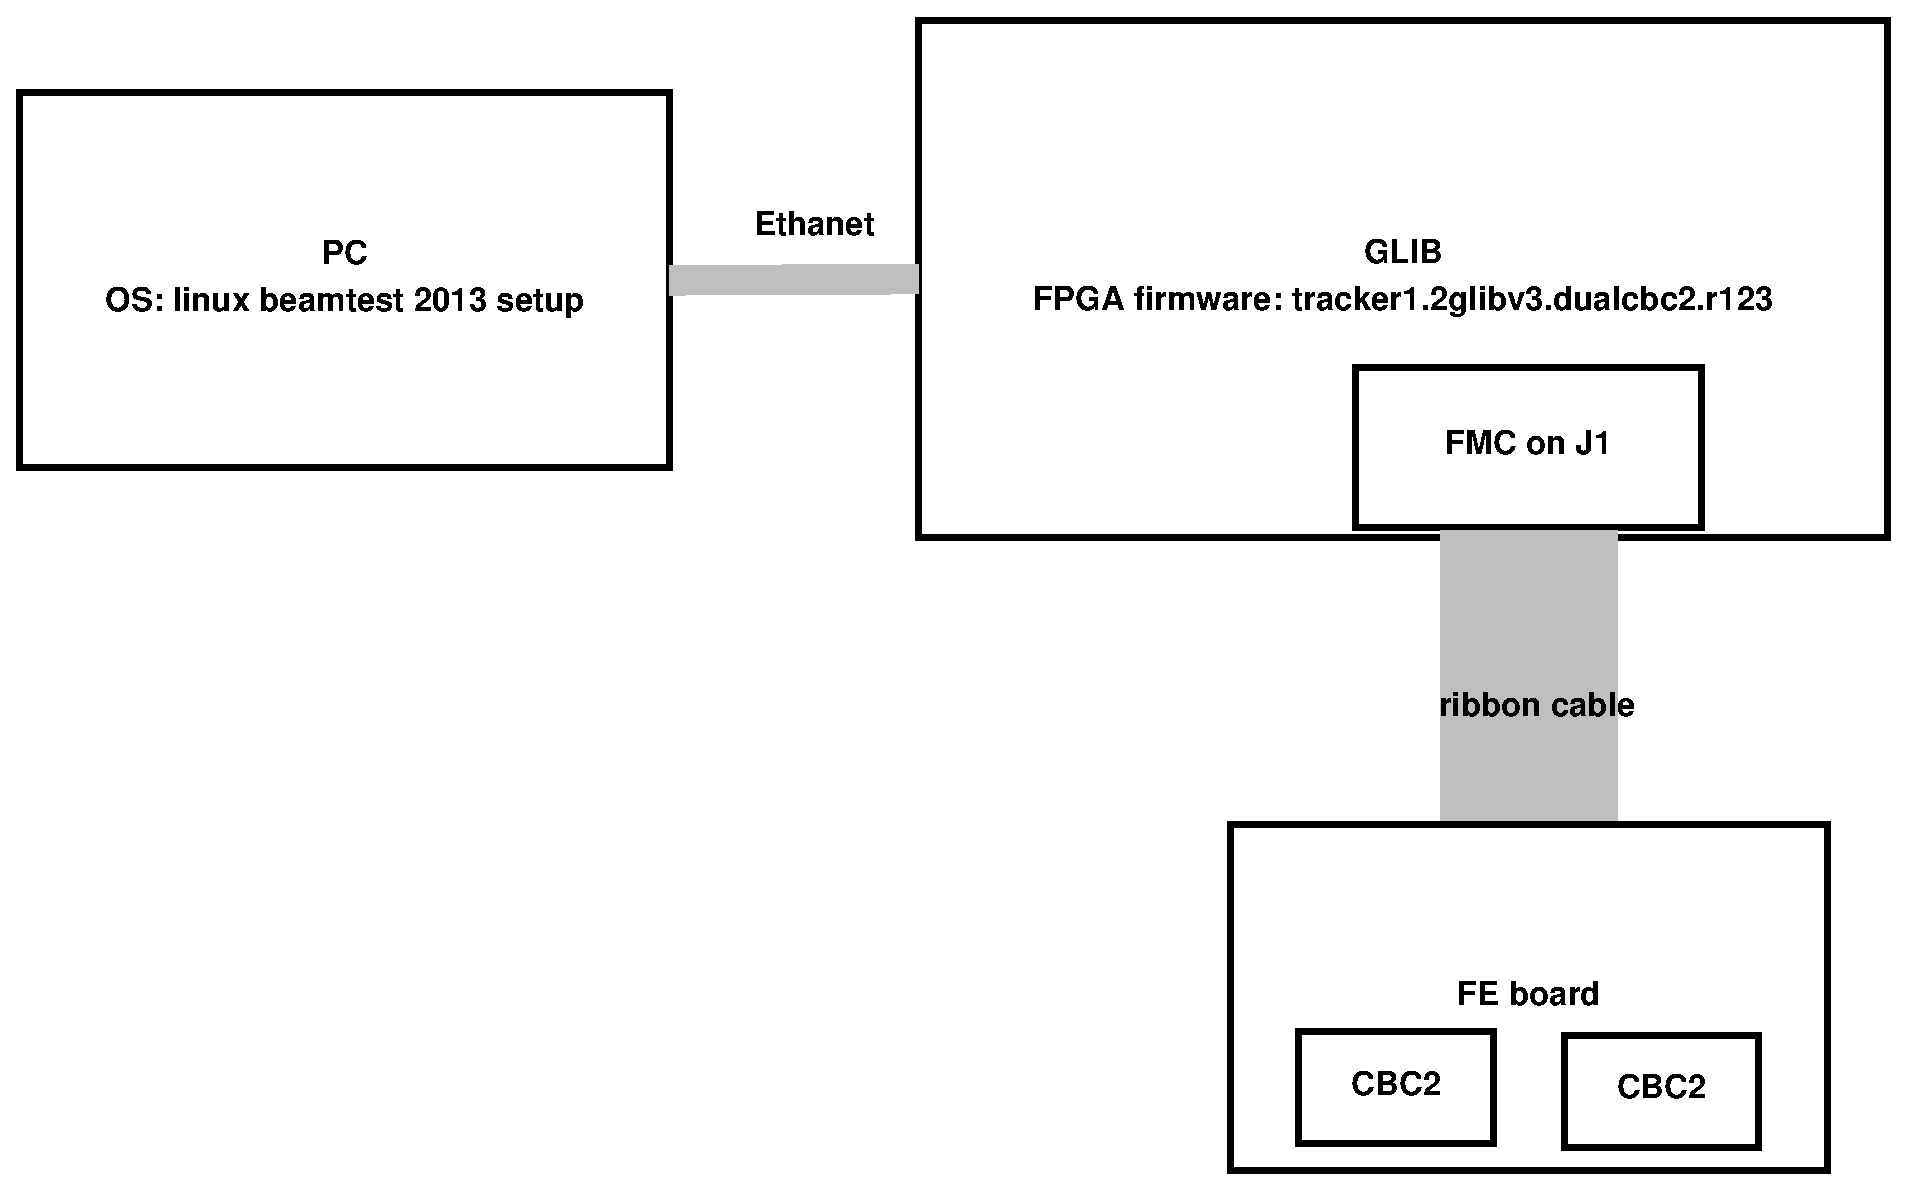
\includegraphics[width=\textwidth]{fig/TestBench.eps}
	%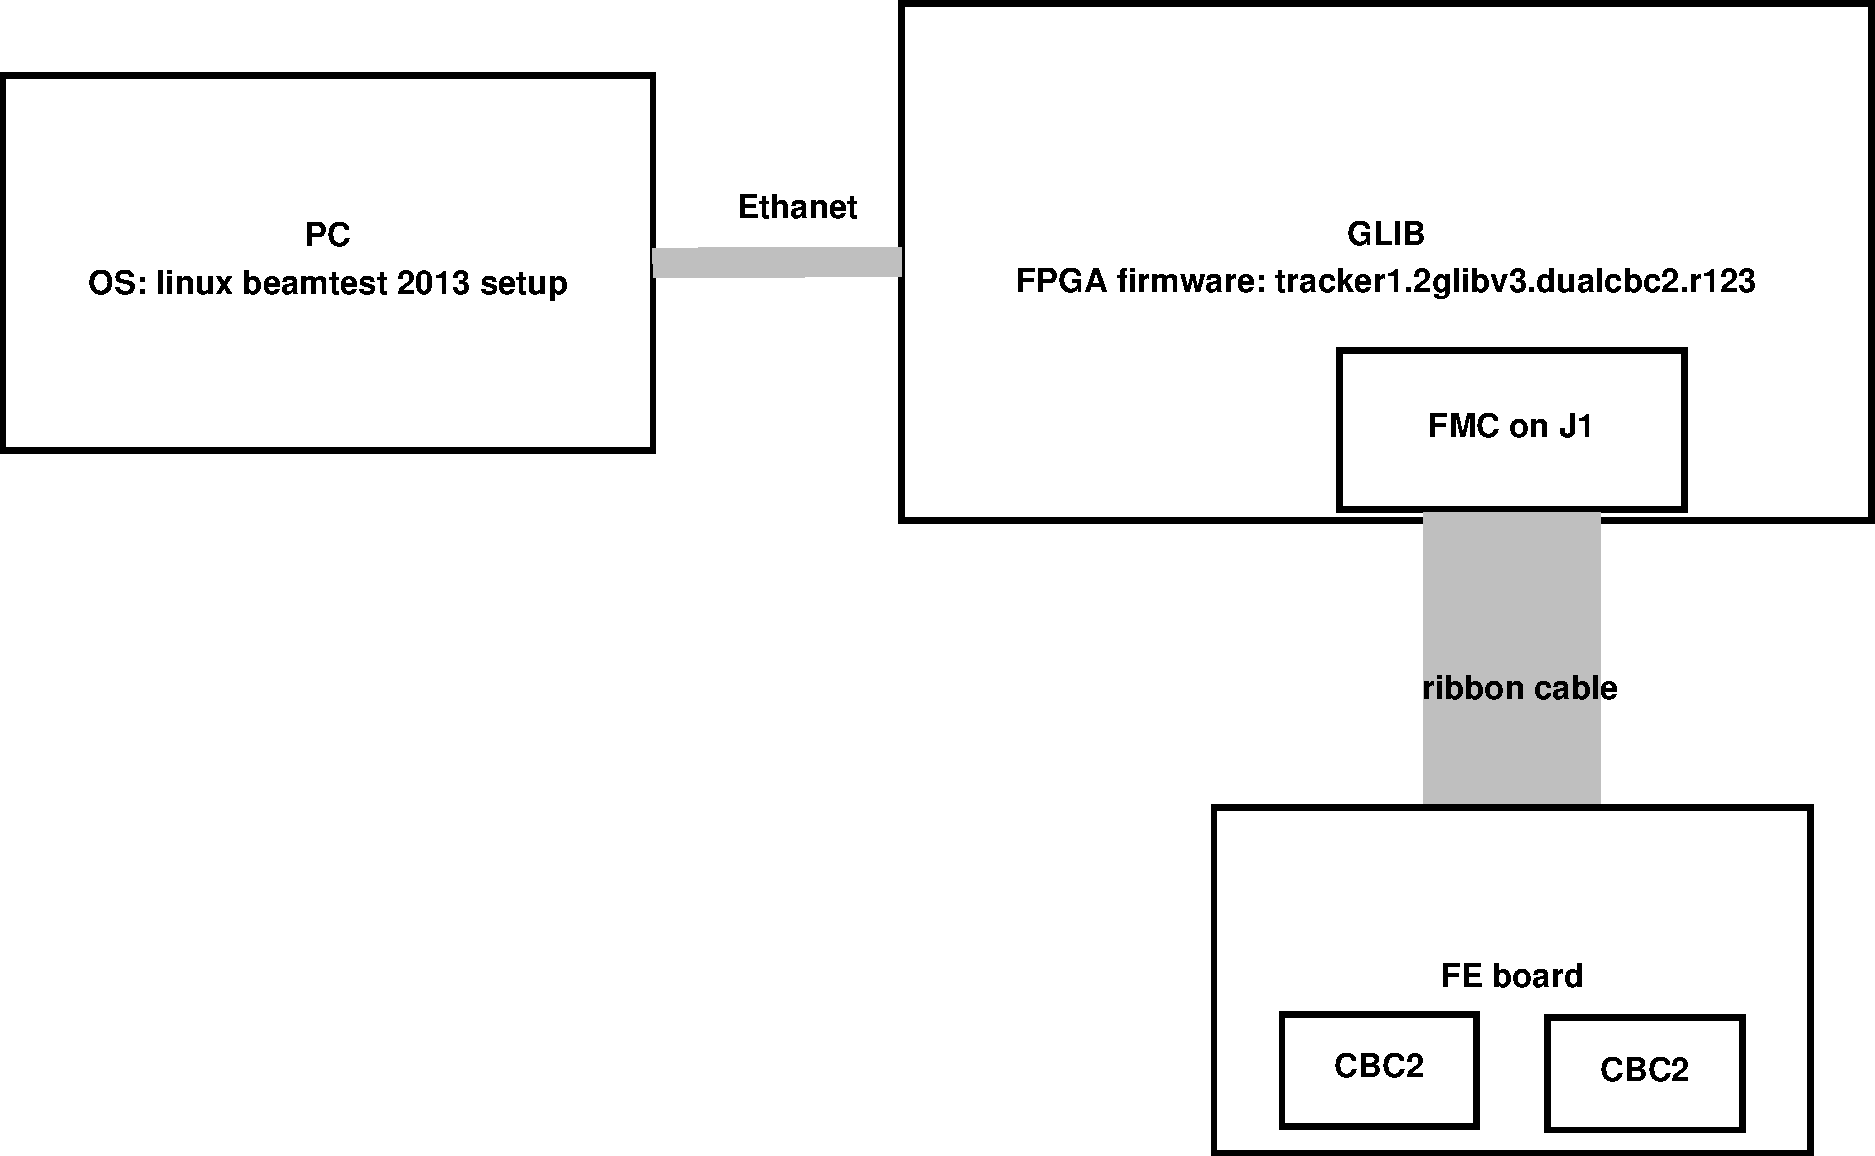
\includegraphics[width=\textwidth]{fig/TestBench.jpg}
	\caption{Testbench diagram. }\label{fig:testbench}
	\end{figure}

	\subsection{Software package: CbcTest}
	The software is coded in C++ using UHAL\cite{UHAL} for the hardware interface (IPBUS) and ROOT\cite{ROOT} is used mainly for histograming and GUI. 
	This is built as a standalone software outside the beamtest DAQ but no additional library is required. The software package is named CbcTest and located at SVN\cite{CBCTEST}. 

	\subsubsection{Structure}
	The CbcTest packages is provided in a compressed tar file, CbcTest.tgz on SVN. Files are extracted with the top directory CbcTest. 
	The CbcTest consist of {\it setup.sh} for environment setting, {\it Makefile} for build, and 10 directories.  
	Four of the directories, {\it utils, Cbc, Strasbourg, and ICCalib} contain source files for each library and the compiled libraries are installed under {\it lib}.
{\it utils} has some useful tools, {\it Cbc} define classes of stractured CBC register data instance, {\it Strasbourg}  is for the interface with Strasbourg's firmware, {\it ICCalib} contains a the proposed calibration sequence and GUI interface.  
{\it src} has calibration and VCTH scan source codes for CUI and GUI using the libraries and executables are build and installed under {\it bin}. 
{\it settings} directory contains some calibration and CBC register settings and {\it macros} directory has some useful ROOT macros for the calibration output root files. 
In the last, {\it doc} directory is for this documentation.   

\subsection{User guide}

\subsubsection{Setup and build}

At the top directory, execute the following commands at bash shell prompt, 
   \begin{quote}
   \verb|source setup.sh|\\
	   \verb|make|
	   \end{quote}
	   After the make, executables are created under bin. In the default setting, the executables are expected to be invoked at the top directory.
	   This is just because the default path for input setting files are set to the relative path \verb|./settings/...|.  The input path can be given as an option
	   in CUI and changed in GUI.

	   \subsubsection{Input setting file}
	   As seen in settings/CbcCalibElectron.txt, the setting file consist of lines with variable name and the value separated by ":".
	   The explanations of the variables are as follows,

	   \begin{description}[style=nextline]
	   \item[GlibConfigurationFile] xml connection file for ipbus.
	   \item[GlibBoardId] the board id in the xml connection file. 
	   \item[BeId] backend board id, used for output directory and histogram names for multiple GLIB settings. 0 or positive number is expected.
	   If this is not given, 0 is used in the software.
	   \item[GlibReg\_CBC\_expected] 1 for 1 CBC and 3 for 2 CBC
	   \item[GlibReg\_COMMISSIONNING\_MODE\_CBC\_TEST\_PULSE\_VALID] Commisioning mode and make test pulse enabled (disabled) on GLIB for 1 (0).
	   \item[GlibReg\_COMMISSIONNING\_MODE\_DELAY\_AFTER\_FAST\_RESET] Number of clock cycle to wait for GLIB to send signal to CBC to generate test pulse after FAST RESET.
	   \item[GlibReg\_COMMISSIONNING\_MODE\_DELAY\_AFTER\_TEST\_PULSE] Number of clock cycle to wait for GLIB to send L1A to CBC after sending signal to CBC to generate test pulse.
	   \item[GlibReg\_COMMISSIONNING\_MODE\_DELAY\_AFTER\_L1A]        Number of clock cycle to wait for GLIB to send FAST RESET to CBC after L1A.
	   \item[GlibReg\_COMMISSIONNING\_MODE\_RQ] GLIB CMMISSIONING MODE request. 1 for calibration data acquisition.
	   \item[GlibReg\_FE\_expected]                                Number of the frontend board.   1 (3) for 1 (2) board.
	   \item[GlibReg\_user\_wb\_ttc\_fmc\_regs.pc\_commands.CBC\_DATA\_PACKET\_NUMBER] Number of event per acquisition.
	   \item[GlibReg\_user\_wb\_ttc\_fmc\_regs.pc\_commands2.negative\_logic\_CBC] 1 (0) for electron (hole) mode.
	   \item[GlibReg\_cbc\_stubdata\_latency\_adjust\_fe1]
	   \item[GlibReg\_cbc\_stubdata\_latency\_adjust\_fe2]         
	   \item[GlibReg\_user\_wb\_ttc\_fmc\_regs.pc\_commands.ACQ\_MODE]
	   \item[GlibReg\_user\_wb\_ttc\_fmc\_regs.pc\_commands.CBC\_DATA\_GENE] 
	   \item[GlibReg\_user\_wb\_ttc\_fmc\_regs.pc\_commands.INT\_TRIGGER\_FREQ]
	   \item[GlibReg\_user\_wb\_ttc\_fmc\_regs.pc\_commands.TRIGGER\_SEL]
	   \item[GlibReg\_user\_wb\_ttc\_fmc\_regs.pc\_commands2.clock\_shift]
	   \item[GlibReg\_user\_wb\_ttc\_fmc\_regs.pc\_commands2.negative\_logic\_sTTS]
	   \item[GlibReg\_user\_wb\_ttc\_fmc\_regs.pc\_commands2.polarity\_tlu]
	   \item[CbcConfig\_FE0CBC0] CBC register setting file for front end board id 0 and CBC id 0 
	   \item[CbcConfig\_FE0CBC1] CBC register setting file for front end board id 0 and CBC id 1 
	   \item[Calib\_InitialOffset] Initial OFFSET value for offset calibration. Leave it to 0x00. The value have to be written in hexadecimal.
	   \item[Calib\_TargetOffset] The target OFFSET value. 0x50 as default. The value have to be written in hexadecimal.
	   \item[Calib\_TargetVCth]   Target VCTH value.  0x78 as default. The value have to be written in hexadecimal.
	   \item[Calib\_VplusMax.]    VPLUS maximum value to scan. 0x90 as default. The value have to be written in hexadecimal.
	   \item[Calib\_VplusMin.]    VPLUS minimum value to scan. 0x60 as default. The value have to be written in hexadecimal. 
	   \item[Calib\_VplusStep]    VPLUS scan step value. 0x10 as default. The value have to be written in hexadecimal.
	   \end{description}

	   Do not change the variables which are not explained above.

	   \subsubsection{calib}

	   \verb|USAGE: calib ( [mode] [setting filename] )|\\
		   The [mode] is either {\it electron} or {\it hole}.
		   If [mode] is not given, electrom mode is invoked. If [setting filename] is not given, 
		   the files under ./settings, CbcCalibElectron.txt (CbcCalibHole.txt) for electron (hole) mode.
		   If those files do not exist, the application still runs with the default setting found in DAQController.cc
		   This command executes the procedure explained in Section \ref{subsec:calib-sequence}.

		   \subsubsection{vcthscan}

		   \verb|USAGE: vcthscan ( [mode] [potentiometer value] [setting filename] )|\\
			   The [mode] is either {\it electron} or {\it hole}.
	If [mode] is not given, electrom mode is invoked. 
If [potentiometer value] is not given, -1 is set (no test pulse)
	If [setting filename] is not given, 
	the files under ./settings, CbcCalibElectron.txt (CbcCalibHole.txt) for electron (hole) mode.
	If those files do not exist, the application still runs with the default setting found in DAQController.cc

	This command scans VCTH and creats the s-curves with all the other registers fixed except for the case when test pulse is disabled. 
	If the test pulse is disabled, the scan is also done for group by group and the same trick is made for other OFFSETs as in the calibration. 

	\subsubsection{calibGUI}

	\verb|USAGE: calibGUI|\\
		calibGUI consists of configuration file setting frame on top, command buttons on the bottom, and seven tabs in the middle, [DAQ\&GLIB configuration], [Log], [CBC register], 
	[Calibration configuration] [Vplus vs. VCth0 Graphs], [Scurve Histograms], and [Data].
	The configuration file can be changed anytime. Write down the file path in the text field and push [Load] button.  Recommended buttons to proceed to the next step are highlighted in orange colour. Other valid command buttons are also accessible if you want.
	The normal sequence is to press "ConfigureGlib", "ConfigureCbc", ConfigureCalibration", in the order and either press "Calibrate" or "VCthScan" after that.
	"Calibrate" executes the procedure explained in Section \ref{subsec:calib-sequence}.
	"VCthScan" scans VCTH and creats the s-curves with all the other registers fixed except for the case when test pulse is disabled. 
	If the test pulse is disabled, the scan is also done for group by group and the same trick is made for other OFFSETs as in the calibration. 
	It is better not to move the top window when the calibration is on going to avoid the ROOT to crash.
	Each tabs are explained as follows.
	\begin{description}[style=nextline]
	\item[DAQ\&GLIB configuration] 
	The GLIB address and ID, and GLIB register values are customised in this tab on the fly.  Press "ConfigureGlib" to configure glib after modifying the values in the fields. After the GLIB is configured, CBC register setting files set in the configuration file (default values if not set in the setting file) are shown in the left and "ConfigureCBC" button is highlighted.  Those can be modified before pressing "ConfigureCBC" button. 
	\item[Log]
	Log is shown in this tab.
	\item[CBC register]
	After pressing "ConfigureCbc" button, the register configuration from the files shown in the 
	[DAQ\&GLIB configuration] tab appear in this tab. Each Front end (FE) tab contains it's own CBC tabs. 
	Each CBC tab has it's setting file name field and this can be modified and "LoadAndSet" button load the setting file and those values are set to the CBC register and the result is shown in the GUI panel.
	All the CBC register values are customised on the fly. 
	Registers in Page 1 are listed with the name, address, the read back value after writing the value to the register in the CBC, and the written value from the left to the right.  
	Registers in Page 2 are listed in the same way but without the name. The right most field is editable.  
	If the arrow is clicked or pressed enter after modifying the value, GUI recognises that those are changed and background color changes to orange.  
	You can edit as many field as you want for all the CBCs at the same time. 
	"UpdateCbcRegisters" button at the top of the [CBC register] tab is to write the values to CBCs and GUI panel is updated.
	If the read back value is different from the set value, the field color turns to red, otherwise returned to white.
	"Reset" button next to the "UpdateCbcRegisters"  resets all the modification made and orange highlights and the values are reset.
	Current CBC register values can be saved with "Save" button next to "LoadAndSet" button in each CBC tab.  
	The file name in the editable file name field is used as the output file name. Please change the file name if you do not want to overwrite the file.

	\item[Calibration configuration]
	Calibration configuration is customised in this tab before pressing "ConfigureCalibration".  
	EnableTestPulse can be set to 1 for VCthScan. This is ignored in Calibration.

	\item[Vplus vs. VCth0 Graphs]
	This tab shows Vplus vs. VCth0 graphs in the step to obtain Vplus value in the calibration. 

	\item[Scurve Histograms]
	All the s-curves from VCTH scan are shown in this tab.

	\item[Data]
	If "Start data stream display" button is pressed, prescaled data stream is shown in this tab.  This slows down the procedure and can be disabled
	any time pressing the same button with the letter "Stop data stream display".

	\end{description}

	\bibliography{CMS_UPGRADE}
	\bibliographystyle{plain}
	\end{document}

